\documentclass{ctexart}
\usepackage{ctex}
\usepackage{amssymb,amsfonts,amsmath,booktabs,upgreek, graphicx,listings,color,xcolor,hyperref}
\hypersetup{
	bookmarks=true,
	bookmarksopen=true
}
\everymath{\displaystyle}
\bibliographystyle{unsrt}
\usepackage[a4paper,left=3.08cm,right=2.68cm,top=2.54cm,bottom=2.54cm]{geometry}
\CTEXsetup[name={,、},number={\chinese{section}},format={\centering\kaishu\zihao{-3}},aftername={\hspace{0cm}}]{section}
\CTEXsetup[format={\raggedright},aftername={\hspace{5bp}}]{subsection}
\CTEXsetup[format={\raggedright},aftername={\hspace{5bp}}]{subsubsection}
%\linespread{1.4}
\lstset{ % 整体设置
    flexiblecolumns,
    %numbers=left,%在左边显示行数
    %numberstyle=\footnotesize,%行数以脚注的大小
	%language=Matlab,
	%frame=true,%显示代码边框
	breaklines=true,
	basicstyle=\small\tt,
	keywordstyle=\color{blue},
	stringstyle=\color[cmyk]{0.45,0.86,0,0},
	commentstyle=\color[RGB]{0,120,2},
	tabsize=4,%设置代码前面的空白长度
}

%导言区

%正文区
\begin{document}\thispagestyle{empty}
    \centering{\yahei\zihao{-2}五一数学建模竞赛}\\
    \bigskip 
    {\yahei\zihao{3}承\ \ 诺\ \ 书}
    
    \medskip
    \raggedright{\zihao{-4}
    我们仔细阅读了五一数学建模竞赛的竞赛规则。
    
    我们完全明白,在竞赛开始后参赛队员不能以任何方式(包括电话、电子邮件、网上咨询等)与本队以外的任何人(包括指导教师)研究、讨论与赛题有关的问题。
    
    我们知道,抄袭别人的成果是违反竞赛规则的, 如果引用别人的成果或其它公开的资料(包括网上查到的资料),必须按照规定的参考文献的表述方式在正文引用处和参考文献中明确列出。
    
    我们郑重承诺,严格遵守竞赛规则,以保证竞赛的公正、公平性。如有违反竞赛规则的行为,我们愿意承担由此引起的一切后果。
    
    我们授权五一数学建模竞赛组委会,可将我们的论文以任何形式进行公开展示(包括进行网上公示,在书籍、期刊和其他媒体进行正式或非正式发表等)。
    
    参赛题号(从A/B/C中选择一项填写):\underline{\hspace{11.7pc}}
    
    参赛队号:\underline{\hspace{10pc}A123456789\hspace{10pc}}
    
    参赛组别(研究生、本科、专科、高中):\underline{\hspace{4.75pc}本科\hspace{4.75pc}}
    
    所属学校(学校全称):\underline{\hspace{6.75pc}嘤嘤嘤大学\hspace{6.75pc}}
    
    参赛队员:
    \begin{tabular}[t]{c}
    	队员1姓名:\underline{\hspace{4pc}嘤嘤嘤\hspace{4pc}}\\
    	队员2姓名:\underline{\hspace{4pc}嘤嘤嘤\hspace{4pc}}\\
    	队员3姓名:\underline{\hspace{4pc}嘤嘤嘤\hspace{4pc}}
    \end{tabular}\\
    联系方式: Email:\underline{\hspace{2pc}123456789@qq.com   \hspace{2pc}}联系电话:\underline{\hspace{2pc}123456789\hspace{2pc}}
    }

    \hfil%空行
    
    
    \raggedleft{\zihao{-4}日期:\underline{\hspace{1pc}2019\hspace{1pc}}年~\underline{\hspace{0.5pc}5\hspace{0.5pc}}月~\underline{\hspace{0.5pc}1\hspace{0.5pc}}日
    \begin{figure}[b]
    	\centering
    	\textbf{\zihao{4}(除本页外不允许出现学校及个人信息)}
    \end{figure}
    
    \newpage%强制换页
    
    \centering{\yahei\textbf{\zihao{-2}五\ 一\ 数\ 学\ 建\ 模\ 竞\ 赛}}
    \thispagestyle{empty}
    \begin{figure}[h]\centering
    	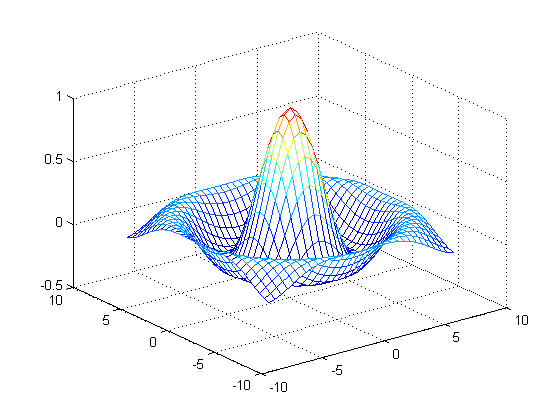
\includegraphics[scale=0.2]{logo.png}
    \end{figure}

    {\zihao{4}\textbf{题\ 目:}\underline{\hspace{22pc}}}
    
    \bigskip
    \centering
    {\zihao{-4}\textbf{摘\hspace{1pc}要}}
    
    \raggedright
    近年来,资源性地区经济转型发展尤为重要,而徐州作为“国家全域旅游
    示范区”首批创建单位,全区游客流量大,路线复杂。本文针对徐州潘安湖风景区
    游览路线问题,根据不同问题的约束,建立不同的游览路线模型,使得在规定时间
    范围内,游客游览时间最长,步行时间最短。
    针对问题一:需要得到从景石出发,到达⑦湿地商业街,且经过①—⑥所有景
    点至少一次的最短路线。使用 Python 程序遍历所有路线,求出各路线中最短的一
    条:景石→③→⑤→①→②→④→⑥→⑦,该路线长度为 1820 米。
    针对问题二:需要为游客设计一条能游览玩全部景点,且游览总时间最长的路
    线。使用 Python 程序遍历所有路线,但是第一个景点不为③森林小剧场,求出各
    路线中最短的一条:景石→②→④→③→⑤→①→⑥→⑦,该路线长度为 2000
    米。
    针对问题三:需要为三个旅游团分别设计一条游览总时间最长的路线,但是一
    个景点同时只能容纳一个旅游团,所以三个旅游团分别要走不同的路线。根据问题
    二可以得出其中一条,第二条路线使用 Python 程序遍历所有路线,但是第一个景
    点不为②阳光草坪、③森林小剧场,求出各路线中最短的一条:景石→①→⑤→③
    →②→④→⑥→⑦,该路线长度为 2040 米,第三条路线使用 Python 程序遍历所有
    路线,但是第一个景点不为①游客服务中心、②阳光草坪、③森林小剧场,求出各
    路线中最短的一条:景石→⑤→③→②→④→①→⑥→⑦,该路线长度为 2100
    米。
    针对问题四:在问题三的基础上,控制旅游团的步行速度,得出两条最短路
    线,景石→②→④→③→⑤→①→⑥→⑦,该路线长度为 2000 米;景石→①→⑤
    →③→②→④→⑥→⑦,该路线长度为 2040 米。长度为 2000 米的游览路线只能有
    一个旅游团行走,长度为 2040 米的游览路线可有两个旅游团行走,使用 Lingo 程
    序求出各个景点的游览时间以及步行速度。
    针对问题五:在问题四的基础上,考虑了两个不确定因素,将旅游团可能的出
    发时间分为五段,根据每段出发时间分配不同的最短路线。建立一个多目标规划模
    型,求出最短路线。
    \medskip
    
   
    \raggedright
    {\zihao{-4}\textbf{关键词}}:Python 语言 \hspace{1pc}Lingo 语言\hspace{1pc} 最优路线模型\hspace{1pc} 多路线分配\hspace{1pc} 无等待时间\hspace{1pc} 多目标规划
    
    
    
    
    
    \newpage
    \centering
    \section{问题重述}
	
	\subsection{问题背景}\thispagestyle{plain}
	\setcounter{page}{1}
	\subsection{问题概述}
	
	\section{模型假设}
	
	\section{符号说明}
	\begin{tabular}{cp{15cm}}
		\toprule
		符号  &  意义\\
		\midrule
		$w$  &  一整天运行所需要使用的最少公交车数量\\
		$w_1$  &  早高峰时段运行所需要使用的公交车数量\\
		$w_{11}$  &  早高峰时段所需使用的单班车数量\\
		$w_{21}$  &  早高峰时段所需使用的双班车数量\\
		$w_0$  &  早高峰时段公交的总运行班次数\\
		$\triangle t_j$  &  早高峰时段第$j$个班次与第$j+1$ 个班次的车
		之间的发车间隔\\
		$w_{1k}^i$  &  依公交行车信息表$1$,将时间分为$4$段,第$k$段里第$i$辆单班车的运行班次数。($k=1,2,3,4$)\\
		$w_{2k}^i$  &  依公交行车信息表$1$,将时间分为$4$段,第$k$段里第$i$辆双班车的运行班次数。$(k=1,2,3,4)$\\
		$X_{ijk}$  &  第$i$辆单班车在第$k$个时段的第$j$个班次\\
		$Y_{ijk}$  &  第$i$辆双班车在第$k$个时段的第$j$个班次\\
		$C_{ik}$  &  第$i$辆公交车在第$k$个时段等待的时间间隔\\
		$C_i$  &  第$i$辆双班车司机的吃饭时间点\\
		$D_i$  &  第$i$辆双班车司机的换班时间\\
		$D_{ik}$  &  第$i$辆公交车在第$k$个时段的行车单程时间\\
		$Z_{ij}$  &  第$i$辆双班公交车的第$k$个班次的单程行车时间\\
		$L_{ij}$  &  第$i$辆双班公交车的第$j$个班次的等候时间\\
		\bottomrule
	\end{tabular}
	
	\section{问题分析}
	\subsection{问题一的分析}
	\subsection{问题二的分析}
	\subsection{问题三的分析}
	\subsection{问题四的分析}\thispagestyle{plain}
	\section{模型的建立与求解}
	\subsection{问题一的模型及求解}
	\subsubsection{建模过程}
	\subsubsection{模型建立}
	
	
	\begin{figure}\centering
		\begin{tabular}[]{l}
			目标函数$\min w_1=w_{11}+w_{21}$\\
			约束条件$\mathrm{s.t.}=
			\begin{cases}
			w_0=\sum_{i=1}^{w_{11}}w_{11}^i+\sum_{i=1}^{w_{21}}w_{21}^i\\
			\sum_{j=1}^{w_0-1}\triangle t_j\leqslant120\\
			3\leqslant\triangle t_j\leqslant5\\
			w_{11}^i=\{0,1\}\\
			w_{21}^i=\{0,1\}\\
			i,j\in\mathrm{N^*}
			\end{cases}
			$
		\end{tabular}
	\end{figure}
	\subsubsection{模型的求解}
	\subsection{问题二的模型及求解}
	\subsection{问题三的模型及求解}
	\subsection{问题四的模型及求解}
	\subsubsection{建模过程}
	\subsubsection{模型的建立}\thispagestyle{plain}
	\begin{equation*}
		\begin{tabular}[h]{l}
		\text{目标函数值:}$X_{ij},Y_{ij},C_{ij},D_{ij}$\\
		\text{约束条件}:
		$\begin{cases}
		\sum_{i=1}^{6}\sum_{j=1}^{n}(X_{ijk}+Y_{ijk})\in[4,6],k=1
		\end{cases}$
		\end{tabular}
	\end{equation*}
	\subsubsection{模型的求解}
    \begin{enumerate}
    	\item 算法
    	\begin{enumerate}
    		\item 先将模型中的一部分约束条件组合在一起,用 Lingo 软件编程得到$2$路公交车排班表;
    		\item 根据排班表可以计算出最少2路公交车使用的最少车辆数以及对应的单双班的车辆数,将此结果与另一部分约束条件进行比较,看其是否符合;
    		\item 若符合,则输出所得结果;若不符合,则再重新选择一部分约束条件,回到~(a).
    	\end{enumerate}
    \item 结果
    
    最少公交车数量为$22$辆,其中单班车为$3$辆,双班车为$19$辆。排班表详见附录$9.2.3$表$1-5$。
    \end{enumerate}\thispagestyle{plain}
	
	\section{模型检验}
	\subsection{问题一}
	\subsubsection{误差分析}
	\subsubsection{结果分析}
	\subsubsection{模型检验}
	\subsection{问题二}
	\section{模型的评价及改进}
	\subsection{模型的优点}
	\subsection{模型的缺点}
	\subsection{模型的改进}
	\section{参考文献}
	%\raggedright
	%\begin{enumerate}
	%	\item[1.1]
		
	%\end{enumerate}
	\newpage
	\section{附录}
	\subsection{问题1的matlab程序}
	\thispagestyle{plain}
	\begin{lstlisting}[language=matlab,%语言是matlab语言
	flexiblecolumns,
	showstringspaces=false]%取消字符间的显示空格
	
        rand('state',sum(clock)); % 初始化随机数发生器
        p0=0;
		tic % 计时开始
		for i=1:10^6
		    x=randi([0,99],1,5); % 产生一行五列的区间[0,99]上的随机整数
		    [f,g]=mengte(x);
		    if all(g<=0)
		           if p0<f
		                x0=x; p0=f; % 记录下当前较好的解
		           end
		    end
		 end
		 x0,p0
		 toc % 计时结束
	\end{lstlisting}
\end{document}